\chapter{Background}

As this thesis is about maintaining differently refactored branchs within a version control system refactoring what follows is some background concerning version control systems and how they determine if a change has occured in source code.  We will also cover refactoring before looking more closely at JDime. JDime is an existing tool that reconciles differently refactored views and reduces merge conflicts. 


\section{Version Control Systems}
Version control systems are a way of managing different revisions (or versions). Version control systems can be used to keep revisions of files that are in any format. Most commonly they are used to maintain source code written for a plain text programming language (e.g. Java, C, etc).   There are a number of reasons why we might want to use a version control system. It can be used to refer to previous revisions, to maintain a revision that has an expirimental feature, to associate additional documentation about a feature or to collaborate with mutiple developers who are on the same programming project.


\begin{description}

  \item [Revist revisions using tagging.]   
    A version control system can be used by a single person to manage different revisions of their program. A previous revision can always be revisited at a later date and changed. If there is something significant about a particular revision it can be labelled with a emph{tag}. A tag assigns a name to all the files in the revision you are interested in so that you can more easily revisit the code at a certain point.  This is helpful if a software package has a number of released versions.  If you need to go back and revisit a particular release it becomes a lot easier if you have tagged the code at that point with the release name or identification.
   
   

  
  \item [Use branching for expirimental features.] 
  It is also possible to maintain mutliple revisions of all the files in a project. This is useful if there is an experimental feature which you want to explore but want to maintain the original project. A version control system can keep these multiple interests separate by putting them on different \emph{branches}.  It is still possible to easily switch between the different branches depending on which project you want to make changes to.  A good use of this feature is if you have a software project that you have written on behalf two different companies but each of them would like their own unique customisations on top of the base product.  By making two copies of the base product and having a record of when it was divided the branches can later be recombined to include some or all of the features that have been introduced.

  \begin{figure}[h]
  \begin{center}
  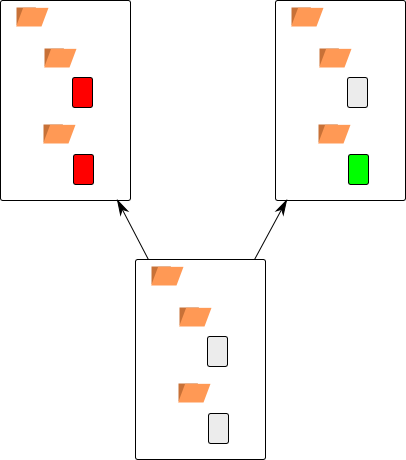
\includegraphics[scale=1]{branching}
  \end{center}
   \caption{A project that has been split into two branches}
  \end{figure}


  \item [Attach documentation to a feature.]    
  Another useful feature of version control is the ability to record meta-information beside a change or a set of changes to a document.  The reason this is useful is that you can specify what the change was for.  Instead of updating individual documents you could specify that changes over multiple documents were done for a single reason.  For instance if you had a number of documents that had an address written in them and that address changes.  Once the change has been made is possible in most version control systems to write a message when the documents are checked in.  In some version control systems this message is required to check-in any set of documents.  The reason this is useful is at a later date if queries are made about what a certain change to a document was for.  Since there is a message beside all the documents about the reason for a particular change it becomes easier to figure out the reason for the individual change we are interested in. If following the example above we were to examine a document and wonder why the address changed we could examine the check in with that change and see the message that the person changing it wrote.

  When used on source code in tandem with an issue tracking system the message can contain the identification number for the bug being fixed or feature being added.  This means that anybody who is examining the revision to see the reasoning for the change has access to a lot more information via the issue tracking system.

  % show screen-shot of Bugzilla
  % 
  % show the commands for adding a comment to git with the Bugzilla number
  % 
  % show how we can get the Bugzilla number back

  \item [Collaborate with multiple developers.]
  Version control systems make it possible to have individual revisions that contain each persons changes. The version control system then manages the way these changes are merged into a composite product. Bertino \cite{Bertino2012} descibes the ability to merge the work of multiple people as being a powerful colabrative tool. This allows multiple people to work on the same document. In some circumstances it allows them to work on the document at the same time.   A version control system allows people with different ideas to collaborate on a single document.

  In order to manage to the different version or revisions version control systems work better on plain text documents. One of the main uses for a version control system is to maintain source code written in a plain text programming language, such as Java or C.

\end{description}



\subsection{Dealing with conflicts}
When people work within the same environment there is a need to interact with each other.
There is competition for access to the source code for each of them to successfully do their work.
There is the risk that they will attempt to change the same block of source code at the same time.
If different changes are made to the same block of source code there is a conflict about what the final can cause a conflict about how the final should be changed.
There are a few ways of dealing with these conflicts.

\subsubsection{Locking}
One approach is to require that the file is only able to be used by one person at a time and that anyone else has to wait. The advantage of this is that the file is always in a consistent state. The disadvantage of this is if one person retains the document for extended periods of time it cannot be changed by anybody else. If a lot of work has been done on the document before it is unlocked for others to edit it.Furthermore the resulting document may be barely recognisable as the original if extensive work is done on it. If the two parties are changing distinctly different parts of the document or change the document in the same way this restriction is unnecessary.

This is how one of the original versioning systems, RCS ensured that the document stayed consistent. Tichy has explained why he considers locking in a version control system to be a good idea in the design for RCS\cite{Tichy1982}

\subsubsection{Smaller structured units}
Another way to reduce conflicts is to split the programming code into smaller units.  The advantage of this is that if you are using locking you minimise the risk that similar. If we go back to the illustration of two people working on the same set of documents.  If instead of one person having sole possession of a document at a time that person only has possession of the page or pages they are changing. As those pages are smaller than the whole document they are likely to retain them for shorter periods.
\subsubsection{Merging documents}
Finally we could allow both parties to change the document and try to figure out what the problems are afterwards.  This resolution of anything that remains a conflict is known as a merge.

If not regularly merged is possible for the source code to diverge greatly and it becomes harder and harder to reconcile.
 According to Bertino it is possible to keep a smaller more easily deployed repository by evaluating what is necessary and what is unnecessary \cite{Bertino2012}. Although Bertino refers to unnecessary files this premise may also be applicable for the smaller blocks of code we are interested in. This suggests that maintaining a record about what is relevant and what is irrelevant may have some benefit. Version control still can have problems with merge conflicts. These issues have a far greater chance of occurring if there is a dramatic change such as refactoring
 
\subsubsection{Manual Merging}


% Manual merge Example
% 
% if you have two document you want to merge but no record of a starting point 
% for them both you will need to manually merge any differences as the 
% computer has no record about what the original document looked like.  
% features that they have in common will not need to be affected however a 
% decision needs to be made about any differences.
% 
% insert diagram

\subsubsection{Automatic Merging}
If there is a three way merge it is possible for the computer to calculate the merge independently provided that there are no merge conflicts.
To do 3 way merging requires 3 different revisions are required, the changes you have made, the changes made by others, and the revision that is common to them both.


% Diagram showing that how merging could be done automatically
% if there is a change in your code but no change in others code automatic
% if there is a change in others code but not yours
% 

\subsection{Architecture}
\begin{description}

  \item [Centralised version control] 
  In a centralised version repository all the changes are made to one location.  This means that only one place needs to be checked in order to access the most up-to-date source code. The need to be connected to a central system solved a lot of issues but often had a large overhead.  In some centralised system it required a specialist to be involved just to look after the server and ensure that merges were done correctly.
  % Still had the model of a central repository everyone needed to consistent  
  % similar to RCS in that you could still check the file out but it was not 
  % as necessary to lock the file  it was possible to look at the differences 
  % between the files and then automatically merge when it was possible  
  % centralised systems have better support for locking.
  % 
  % 
  %  examples of centralised systems
  % RCS, CVS, SVN, Clearcase
  % 
  % difference between centalised version controls
  % According to \cite{Bertino2012} centralised version control systems...

  \item [Distributed version control] 
    

  @% mobile access  % @c  % The benefits and costs of distributed systems have long been discussed  %   % examples of distributed version control  % GIT, Mercurial, Bazaar

  difference between git and mecurial reference
  \item [Online version contol systems]  
  Whilst is is possible for a measure of collaboration just by using git on it own it requires that you have some method of obtaining the seperate branches on one machine before they can be merged.  One way of doing this within a company is to set up a git server.  This might suitable for projects that are closed source and have a select group of people who work on the source code.  For larger projects that have has programmers in different parts of the world a publicly accessible git server that is on the web may be a better solution.    
  % the reason i achieve included this here is because the amount of   % interaction in git means that merge needs to be better  % add a screen shot to show the number of forks an users of a large project\end{description}

  
\end{description}

\section{Longest Common Subsequence}
The longest common subsequence problem isThere are a number of issues in computer science that can be resolved by a longest common subsequence algorithm.
It is very good at finding the differences between two different sets of ordered information.

% look into other uses for LCS

\subsection{Example}
One method of discovering what has changed is to find the longest common subsequence (LCS).
A simplified example of finding the longest common subsequence is:

Imagine we have have two similar sets of java source code that we want to compare with each other.  
We would like to know what is the same and what is different.
A longest common subsequence for the source would contain a list of all the lines that are the same and in the same order.

The first listing is as follows:

\begin{lstlisting}
public class SampleLCS { 

  public static double area(double radius){
    return Math.PI * square(radius);
  }
  
 public static void main(String[] args){
   System.out.println(area(3));
 }
 
 public static double square(double num){
   return num * num;
 }
}

\end{lstlisting}

In the second listing the order of a number of methods has changed but the way the code works has not been changed.

\begin{lstlisting}
public class SampleLCS {

 public static void main(String[] args){
   System.out.println(area(3));
 }
 
 public static double square(double num){
   return num * num;
 }
 
 public static double area(double radius){
   return Math.PI * square(radius);
 }
}

\end{lstlisting}

A listing containing only the common lines in the same order between both listings follows.  If this is the longest listing possible it is known as the longest common subsequence.  

\begin{lstlisting}
public class SampleLCS { 

  public static double area(double radius){
    return Math.PI * square(radius);
  }
  
}

\end{lstlisting}

It is possible to have more than one longest common subsequence if there are multiple listings of common lines that have the same number of lines in common and have the maximum number of lines that match.  For instance the following listing is also a longest common subsequence of the above example.

\begin{lstlisting}
public class SampleLCS {

 public static void main(String[] args){
   System.out.println(area(3));
 }
 
}
\end{lstlisting}

As there are possibly multiple longest common subsequences identifying the longest common subsequence that is going to be most useful becomes difficult.

\subsection{Methods of calculating LCS}
According to Arslan \cite{Arslan2010} there are many algorithms that solve longest common subsequence problem. The algorithms used in JGit for example are the the Myers, Patience and Histogram algorithms.

\subsection{Myers}
The Myers algorithm was discovered by Eugene Myers who claimed that finding the minimal differences between any two documents was the equivalent to finding the shortest or longest path in a graph \cite{Myers1986}. 

\subsection{Patience}
The patience algorithm instead of figuring out the longest common subsequence directly uses the longest increasing subsequence.
When this is used with line numbers from the source code the longest common subsequence can be established.
By examining only unique lines present in both copies of source code it is comparing. it ignores items that are repeated multiple times as they produce longest common subsequence could give a sub-optimal result.

bran Cohen

because of the way a patience 

Before the act
% from the patience game
% need references

\subsection{Histogram}
A Histogram difference strategy is very similar to a patience algorithm
Instead of looking at just the unique lines between any two subsets however it can examine lines that there are multiple copies of 

\subsection{The problem with LCS}
There is still a problem with longest common subsequence. It does not notice changes of order in a document.  For the example we have been looking at two methods have swapped positions.  The program still behaves in the same manner when it is run.  It is unnecessary to make any changes to this code in order to get them to behave the same way. Diff tools that solely use the longest common subsequence do not take different ordered items into account even if they can be considered equivalent.

\begin{figure}[h]
\begin{center}
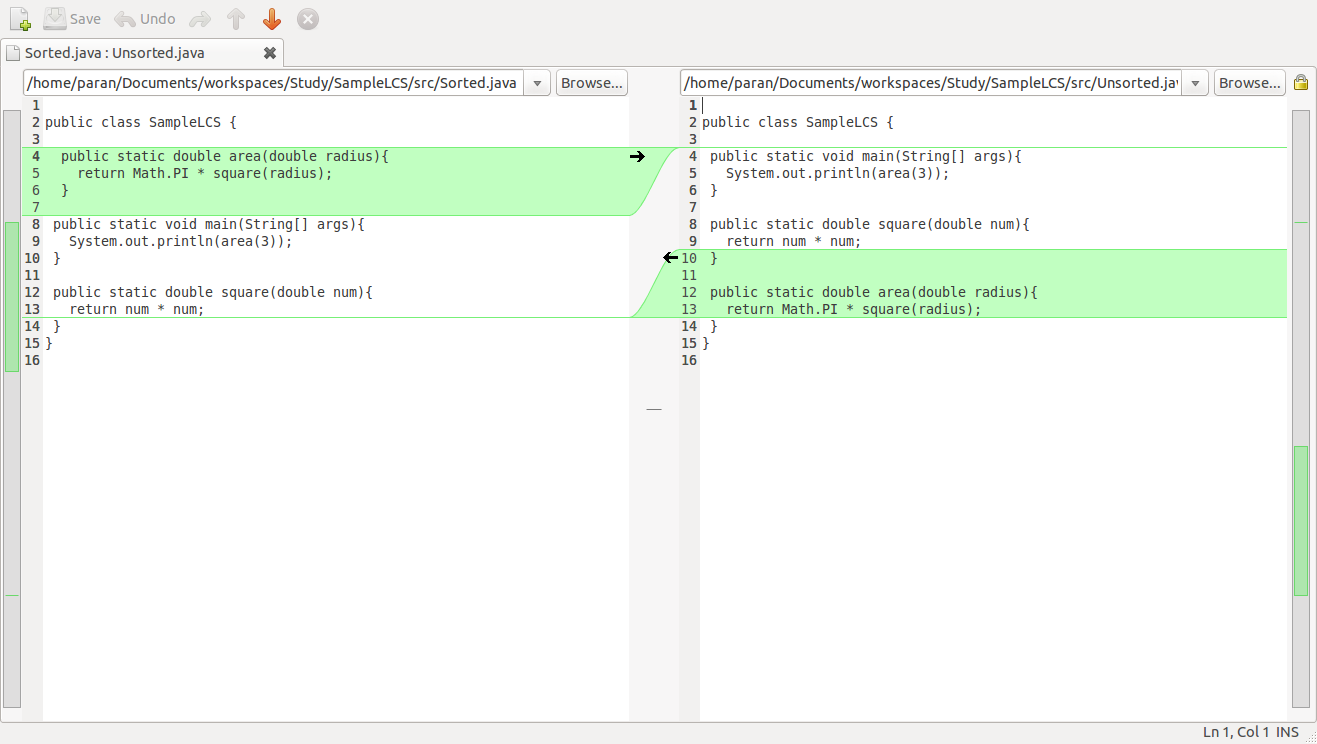
\includegraphics[scale=.25]{lcsDiff}
\end{center}
 \caption{A graphical diff tool showing differences with two equivalent blocks of source code}
\end{figure}

\subsection{How LCS is used in differencing tools}
Often to speed up the differencing process each line is assigned a hash code depending on its contents. 
This means that the differencing tool can work much faster as it does not need to compare each character in the line but can compare hash codes instead.
In the source code for many programming languages the white space is not relevant so many diff tools have the option of ignoring the white-space and only comparing the code.
This has an impact on the hash codes for each line as the hash code needs to be generated just from the text rather than the white spaces in the code.
% Remember to say something white space
% and regular expression differences
% 
 

\section{Refactoring}

A common concern with coding is the need to periodically refactor the code. Refactoring does not involve changing any of features the source code or change how the compiled program functions. Refactoring simply reorganises the source code so that it is easier to read and add changes. According to Fowler et al. the main time for refactoring is when new functionality is added \cite{Fowler1999}. Similarly according to Kerievsky some of the motivations for refactoring include adding more code and understanding existing code \cite{Kerievsky2004}. As adding more functionality is one of the motivations for refactoring let us consider what happens in a multi-developer environment. Two developers could have different views on what is considered an appropriate refactoring. This is especially true if they need to add different functionality from each other. 

A simple example is illustrated as follows:

\begin{lstlisting}
public TempConv() {
  Scanner keyboard = new Scanner(System.in);
  System.out.println("Enter the temperature in Celsius");
  int celsius = keyboard.nextInt();
  System.out.println("Degrees Fahrenheit is approx " 
    + (celsius * 2 + 30) );
  keyboard.close();
}
\end{lstlisting}

Refactoring this code depends on what functionality you need to add. One developer may recognize that conversion from Celsius may be used several times throughout the code and so extract the calculations as a separate method as follows:

\begin{lstlisting}
public TempConv() {
  Scanner keyboard = new Scanner(System.in);
  System.out.println("Enter the temperature in Celsius");
  int celsius = keyboard.nextInt();
  System.out.println("Degrees Fahrenheit is approx " 
    + celsiusToFahrenheit(celsius));
  keyboard.close();
}

public int celsiusToFahrenheit(int celsius){
  return celsius * 2 + 30;
}
\end{lstlisting}

This change, in spite of producing the same output as the first, provides a number of advantages. Firstly if other programs need to convert from Celsius to Fahrenheit the new method can easily be reused. Secondly since the calculation is a crude estimation it becomes a lot clearer where the code needs to be changed to improve the formula. The ability to add a method that clearly indicates that the calculation is from Celsius to Fahrenheit helps with the readability of the code. There are also disadvantages to doing this refactoring however. If we do not care about conversion between Celsius and Fahrenheit the refactoring simply adds to the amount of code we need to wade through before understanding what the code does. An alternate way of refactoring is as follows:

\begin{lstlisting}
public TempConv(){
  Scanner keyboard = new Scanner(System.in);
  System.out.println("Enter the temperature in Celsius");
  int celsius = keyboard.nextInt();
  int celsiusToFahrenheit = celsius *2 + 30;
  System.out.println("Degrees Fahrenheit is approx " 
    + celsiusToFahrenheit);
  keyboard.close();
}
\end{lstlisting}

While this again expresses the same functionality as the code above it has not created a new method to do so. This has some of the same advantages. It separates and identifies the formula to convert between Celsius and Fahrenheit. It also uses less code to express this separation than forming a new method. It does not expose the conversion formula outside this method to be used by other calculations however.

As the value of a particular refactoring appears to depend on what is trying to be achieved it is very hard to claim that one refactoring is better than another. It depends entirely on the wider context of the intention for the refactoring, in this case the level of access required for the approximation to convert Celsius to Fahrenheit.

Although this was a simple example it is easy to imagine a case where a much larger refactoring process is undertaken. In such circumstances a merge becomes difficult. 

\section{JDime}
Part of the inspiration for this tool come from JDime. If there is a conflict in a text based merge JDime provides a way for some refactored content to be merged.  

\subsection{What Jdime can be used for}
JDime can be used to compare two different versions of Java source codes which have been refactored and to produce a copy common to them both. 

\subsection{How Jdime works}
JDime instead of testing against a source code repository test against files in the system under the base, left and right directories.
While this may be useful in quickly being able to show what JDime is able to achieve it requires that the inputs need to be previously extracted from a repository into the file system.

Before doing any calculations, JDime runs a regular text merge over the source code.  
If the regular text merge has conflicts then JDime parses the file into an abstract syntax tree (AST).  JDime uses the AST to determine if sections of the source code need to be in a particular order or could be in any order.
What then happens depends on if order is required in the section of code JDime is examining.

\subsection{Testing Jdimes suitability}

Jdime has been written mostly in Java by Apel and Les{\ss}nich \cite{Apel2012} .  There are a few exceptions including the linear programming libraries that need to be created.  As we are attempting to combine some of their work with Git it was decided to use JGit rather than the C implementation of Git. As the Java implementation may run a bit slower then in order to get a good timing test running we need to run redo the tests of JDime using JGit instead. 

Also the tests that Le{\ss}nich did on JDime were from files rather than from a repository. It is necessary to set the files back up in the original repository structure to get a adequate baseline.

As JDime performs a type of automatic merge it requires 3 different revisions.
JDime requires a revision that has changes that we want included.  This is commonly called the right revision however I will call this the merger revision as the changes in it are meant to be merged.
JDime also requires a revision that we want to merge into.  This is commonly called the left revision, however I will refer to this as being the mergee. 
Finally JDime requires an original revision that both the merger and the mergee are based on.
This is commonly called the base revision.

At the moment it cannot access a version control system so each of the revisions need to be set up as directories.
Each directory needs a full copy of the source code for that revision 
This means that the necessary Java source code to be used by JDime in base, left and right directories.


In order to show how JDime performs extra refactoring based merging we need to attempt to try something that would incorrectly cause a conflict in a text based merge.  The reason that this is necessary is that if there are no conflicts in a text based merge the refactoring aware portion of JDime will not be run.  This saves the overhead of loading the program into an AST in the event that the initial text merge has no conflicts. 
One way to get a lot of text conflicts between two pieces of code that are equivalent when they run is to change the order of the methods.
Although the methods are in different order the programs are still \"functionally equivalent\".
In order to examine how JDime works and test its suitability a test handler was written.
The test handler creates all of the directories and files for JDime to process.
The methods inside the files are reordered differently for both the left and the right directories.

\begin{figure}[h]
\begin{center}
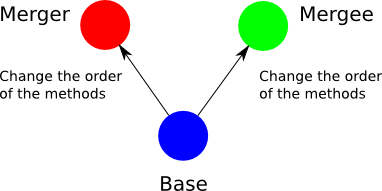
\includegraphics[scale=1]{JdimeTestSetup}
\end{center}
 \caption{The setup for the test of JDime}
\end{figure}

Once the test was set up using the test handler the JDime run to process the directories.
What we expected to happen was that JDime would reorder the methods to match the order in the mergee. When we compared the methods using a graphical merge tool however we found that the order of the methods in the files did not match.

\begin{figure}[h]
\begin{center}
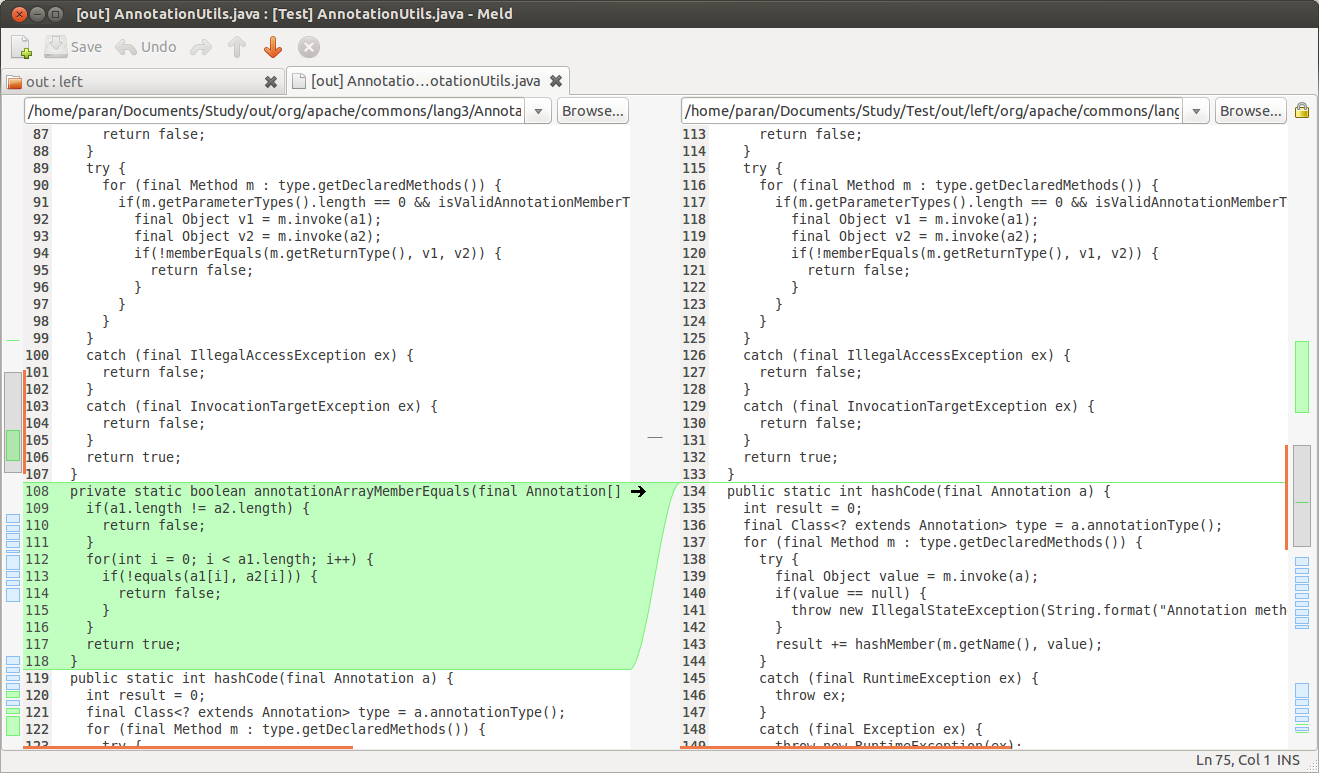
\includegraphics[scale=0.25]{DiffLeft}
\end{center}
 \caption{Screen-shot of Meld showing a different method order}
\end{figure}

It is about this point in analysis that you begin to second guess yourself.  For this reason the output of JDime was compared also with the merger and the base.  The order of the methods in the output did not match the order of any of the equivalent input files.  

If it detects an unordered section it does not preserve the order of the output.

\subsection{Resons why Jdime cannot currently be used to create seperate views}
The aim of this thesis is to be able to maintain two views of Java that although having a different format function in the same manner.  Although this tool sounds like it would be able to help achieve those aims there are a few reasons why it cannot be used without changes.

The first issue is that as explained above that the resulting code could be in a totally different order to any of the versions combined to create it.

The second issue is that when JDime parses the code into an AST it strips out any comments or white-space placed in the code.  Although the comments do not have any functional impact on how the program runs they do have an impact on how the source code is understood.  To limit the impact a merge makes on one view comments need to be evaluated as well. In some ways retaining comments or even white-space in the code aids in determining if a section of the code has been copied verbatim from one place to another.

The only time an AST based merge is performed is if there are conflicts.  There could be advantage to determining if items that haven't conflicted in the text based merge but have moved from one position in the code to another.  If a method has both been moved and changed in both branches it could have a conflict.  This conflict would appear to the text-merge as a deletion agreed upon by both branches followed by two insertions at different points.  It would not be picked up by the text-merge as containing a conflict even if one was potentially present.  Since the conflict is not detected by a text-merge it is not set aside for testing by examining the AST tree. In this case comparing AST trees could detect that there was a conflict. Although JDime is an improvement over a text-based merge this is a potential conflict that niether detect. There is a performance reason for this design decision. JDime can take a long time to determine if two files contain equivalent source code.

The final concern is that after JDime does the initial comparision of text and finds conflicts it discards those results. It parses the entire file into an AST and begins analysing it again without knowing which parts differ.   







\section{Other refactoring aware versioning tools}
JDime is not the only tool that can be used to address refactor aware version control.  Ekman and Asklund \cite{Ekman2004} introduced a plugin for eclipse that recorded information about refactoring in to version control so that it was eaiser to recognise where refactoring took place.  They did this in a very similar manner as Apel and Le{\ss}nich when they developed JDime.  Both make use of ASTs to record information about any refactoring that took place.  Freese \cite{Freese2006} also developed a tool that was very similar written in Object-Z. Despite this interest in refactoring aware merges however the idea of keeping separate branchs as consistant as possible has not been discussed.
 
 


